% Metódy inžinierskej práce

\documentclass[10pt,twoside,slovak,a4paper]{article}

\usepackage[slovak]{babel}
%\usepackage[T1]{fontenc}
\usepackage[IL2]{fontenc} % lepšia sadzba písmena Ľ než v T1
\usepackage[utf8]{inputenc}
\usepackage{graphicx}
\usepackage{url} % príkaz \url na formátovanie URL
\usepackage{hyperref} % odkazy v texte budú aktívne (pri niektorých triedach dokumentov spôsobuje posun textu)

\usepackage{cite}
%\usepackage{times}

\pagestyle{headings}

\title{Názov\thanks{Semestrálny projekt v predmete Metódy inžinierskej práce, ak. rok 2015/16, vedenie: Meno Priezvisko}} % meno a priezvisko vyučujúceho na cvičeniach

\author{Meno Priezvisko\\[2pt]
	{\small Slovenská technická univerzita v Bratislave}\\
	{\small Fakulta informatiky a informačných technológií}\\
	{\small \texttt{...@stuba.sk}}
	}

\date{\small 30. september 2015} % upravte



\begin{document}

\maketitle

\begin{abstract}
	Statická analýza je proces, pri ktorom je počítačový kód zanalyzovaný bez samotného spúšťania kódu.
	Po tejto procedúre, sú programátorovi prezentované nájdené chyby, ich možný spôsob opravy a aj varovania
	o menej závažných nedostatkoch a ich riešenia. Pomocou tejto metódy dokážeme v celom analyzovanom projekte
	zlepšiť kvalitu kódu a udržať konzistentný štýl, ktorý taktiež spĺňa osvedčené postupy pri vývoji softvéru.
	Veľkou výhodou je tiež urýchlenie hľadania chýb a softvérových defektov v porovnaní s manuálnou kontrolou.
	V tomto článku pochopíme, prečo developeri používajú nástroje statickej analýzy, ako ich používajú
	na opravu a zlepšenie kódu a ako ich implementujú do ich pracovného prostredia.~\cite{Main}
\end{abstract}


\pagebreak






\begin{table}
	\begin{center}
		\begin{tabular}{c|c|r}
			$ID$ & $Krajina$      & $Obyvatelia(mil)$ \\
			\hline
			1    & India          & 340               \\
			2    & USA            & 200               \\
			3    & Indonesia      & 140               \\
			4    & Brazilia       & 130               \\
			5    & Mexiko         & 98                \\
			6    & Filipiny       & 88                \\
			7    & Vietnam        & 54                \\
			8    & Egypt          & 47                \\
			9    & Banglades      & 46                \\
			10   & Pakistan       & 45                \\
			11   & Kolumbia       & 38                \\
			12   & Velka Britania & 38                \\
			13   & Turecko        & 37                \\
		\end{tabular}
		\caption{Tabulka}
		\label{tab:Tabulka 1}
	\end{center}
\end{table}


%{\centering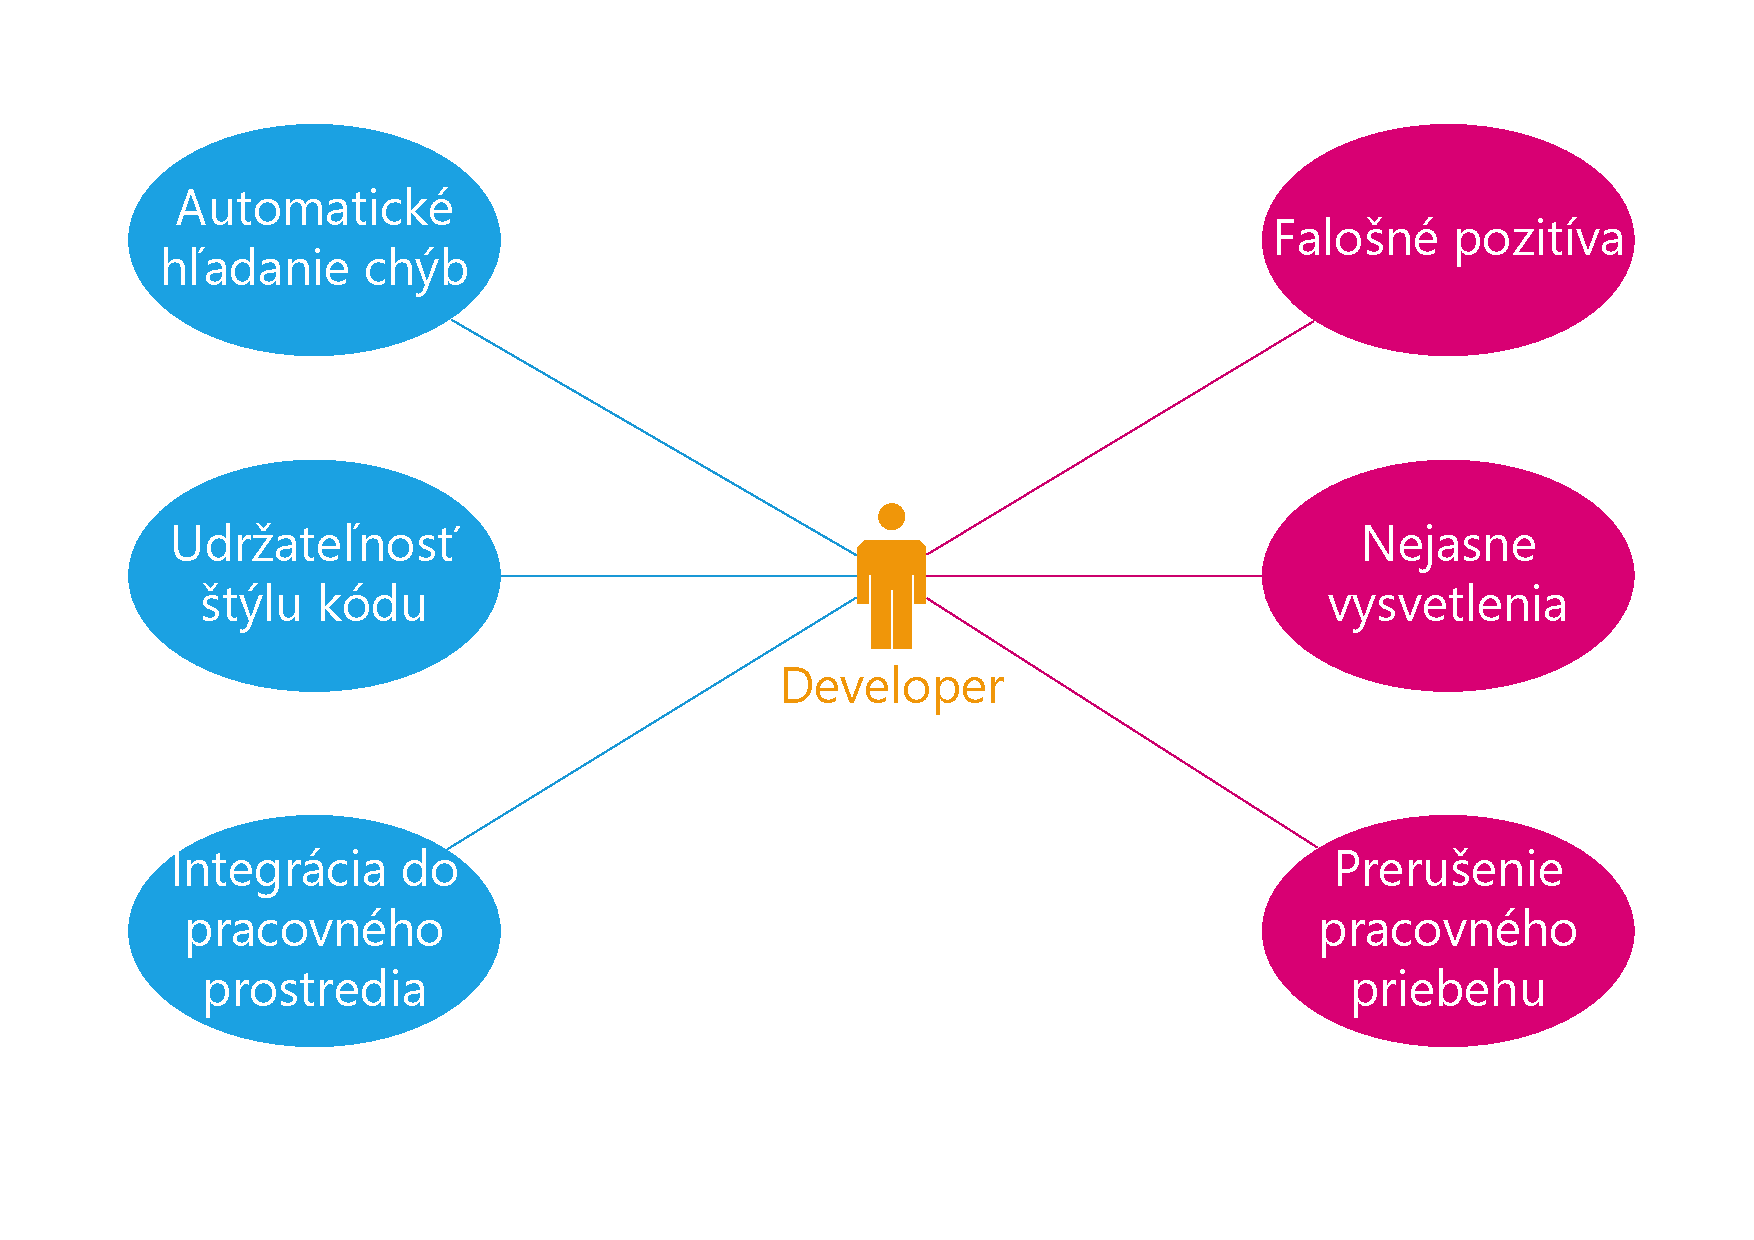
\includegraphics[scale=0.4]{pozitiva_negativa.pdf}}


% týmto sa generuje zoznam literatúry z obsahu súboru literatura.bib podľa toho, na čo sa v článku odkazujete
\bibliography{literatura}
\bibliographystyle{plain} % prípadne alpha, abbrv alebo hociktorý iný
\end{document}
